\section{Convergence of the self-consistent fields}
\label{sec:convergence}


\begin{figure}[t]
    \begin{subfigure}{0.45\textwidth}
        \centering
        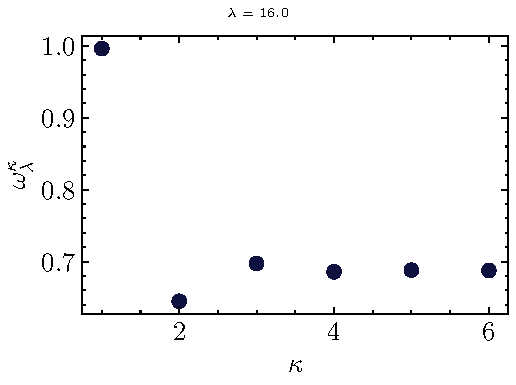
\includegraphics[width=\textwidth]{Figures/convergence/eigenvalues_lambda_16_dirichlet.pdf}
    \end{subfigure}
  \begin{subfigure}{0.45\textwidth}
        \centering
        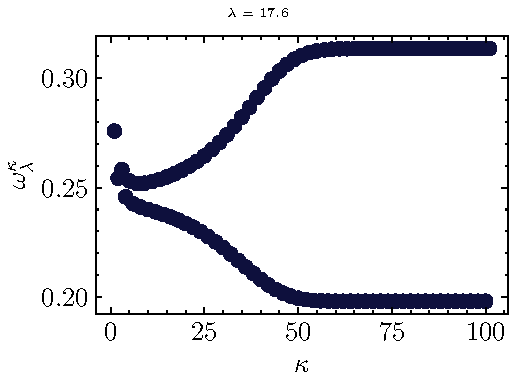
\includegraphics[width=\textwidth]{Figures/convergence/eigenvalues_lambda_17.599999999999998_dirichlet.pdf}
    \end{subfigure}
        \caption{$\omega_1$ of the massless scalar field with DBC for different values of $\lambda$ as a function of the iteration $\kappa$.}        \label{fig:convergence}

\end{figure}

The iterative procedure either
    converges,
    oscillates, or
    breaks down. 
    
The convergence of the iterative procedure described in Sec.~\ref{sec:The-iterative-procedure} is measured through the sequence $\{\omega_{1, \lambda}^\kappa\}_{\kappa>0}$. Examples of a converging sequence and an oscillating (non‑convergent) sequence are displayed in the top and bottom panels of Fig.~\ref{fig:convergence}, respectively. These cases can be understood from the perspective of fixed‑point theory, where we explicitly see whether the update function $f_{\lambda,c}$ is a contraction (top panel) or not (bottom panel).  We conjecture that one can always find a small enough $c$ such that the map $f_{\lambda,c   }$ is contracting.

The iterative procedure breaks down when complex $\omega$ appear. This happens if the candidate $\lambda +\Delta \lambda $ in the numerical continuation method is too far away from $\lambda$: the screening due to $\rho_\lambda$  is too weak compared to $A_{0, \lambda+\Delta \lambda}^1$, and the system effectively behaves as in the external field approximation with $\lambda>\lambda_c$.
The step $\Delta \lambda$ is reduced and the iterative procedure is tried again. 

% \begin{subfigure}{0.5\textwidth}
%     \centering
%     
\includegraphics[width=\textwidth]{subfigures/convergence/eigenvalues_lambda_12_dirichlet.pdf}
%     \caption{$\omega_1$ of the massless scalar field with DBC for $\lambda=12$ (weak-field regime) as a function of the iteration $\kappa.$  }
%     \label{fig:weak-field}
% \end{subfigure}
